\chapter{Grundlagen}

\section{Verwandte Werke}
Bussman et al. erklärt in \cite{Bussmann2006} Impulse, die durch neue Technologien ausgelöst werden können. Dabei wird auch auf die damit verbundene mögliche Modernisierung von Anwendungen im Finanzdienstleistungsbereich eingegangen. Diese wird durch einen Ansteig der Anforderungen in produktionsnahen, operativen Systemen \cite{Bussmann2006, Brockhoff2006} bedingt. Hierfür nennt er zwei spezifische Ansätze. Danach wird die Rolle der IT-Architektur in Verbindung mit der IT-Strategie beschrieben und eine hohe Flexibilität und Schnelligkeit gefordert. Für eine kontinuierliche Anpassung der IT-Architektur, die für den Erfolg wichtig ist \cite{Bussmann2006}, werden die damit verbundenen Schwierigkeiten genannt. Anschließend werden in einem Ausblick große Auswirkungen der IT auf die etablierten Geschäftsmodelle erwartet. Die Ergebnisse von Bussman et al. sind sehr relevant, da die Auswirkungen von neuen Technologien auf das Geschäftsmodell vorausgesehen werden und Bedingungen für den Umgang mit Technologientrends gestellt werden.
\medskip
\\
Brockhoff beschreibt in \cite{Brockhoff2006} die Hintergründe und Probleme der IT-Architektur in Banken und stellt Anforderungen an ihre IT-Architektur. Dabei fordert er die eine \ac{SOA}, um die mangelnde Flexibilität und Skalierbarkeit der alten Architektur zu beseitigen. Die Schilderungen von Brockhoff geben die Probleme in der unflexiblen IT-Architektur aus Sicht des Finanzwesens wieder.
\medskip
\\
Gupta und Simonds beschreiben in \cite{Gupta:2017} Goldman Sachs' Weg der digitalen Transformation hin zu einem Technologieunternehmen und Plattform. 
Die Studie von Gupta und Simonds stellt viele Ansätze vor, mit denen Goldman Sachs erfolgreich neue Geschäftsmodelle entwickelt hat und alte Modelle Strukturen abgeschafft hat. Diese Ansätze könnten als Positivbeispiel für das deutsche Finanzwesen dienen.
\medskip
\\
Disterer beschreibt in \cite{mci/Disterer2011} eine problematische Inbetriebnahme von Anwendungen durch die mangelnde Beachtung von nichtfunktionalen Anforderungen bei der Entwicklung. Hierzu stellt er als Lösungsansatz eine Erweiterung eines ITILv3 Prozesses mit Quality Gates, die als Synchronisationspunkt für die Koordination zwischen Entwicklung und Betrieb dienen. Der Ansatz von Disterer gibt eine Referenz für eine bessere Koordination zwischen Entwicklung und Betrieb.
\medskip
\\
Alt et al. erklärt bezogen auf das IT-Management in \cite{Alt2017} das Potenzial von DevOps zur Steigerung der Innovationsfähigkeit. Dieser ergibt sich aus Kontinuitätskonzepten und ihrer Verbindung mit einer inoovationsfokussierten IT-Strategie. Hierfür erklärt er die DevOps Prinzipien, worin er für das Kontinuitätsprinzip auf den Ansatz \emph{Continuous Delivery} eingeht. 
\medskip
\\
Pathania zeigt in \cite{Pathania2017} wie Jenkins mit Kubernetes, Docker und Public-Cloud skaliert werden kann. Dabei konfiguriert er Jenkins für die Nutzung innerhalb einer Public-Cloud und Kubernetes. Er veranschaulicht einen Ansatz, um den Jenkins Master über Replikas zu skalieren. Zudem beschreibt er die Skalierung von Jenkins Agenten für die Verteilung der Builds. Für die Agenten werden Images erzeugt, woraus Jenkins mithilfe eines Docker Plugins einen Container für den Build generiert. Für die Agenten erstellt er ein Image aus Ubuntu und installiert die Build-Tools, wie in jedem anderen Ubuntu System.
Dadurch erzeugt er die Images über einen Container, welches vorher konfiguriert wurde. Insbesondere beschreibt Pathania ausführlich die einzelnen Schritte, die für die Orchestrierung der ganzen Anwendung mit Kubernetes erforderlich sind.

\section{Stand der Technik}
Zuletzt hat sich die IT vor allem durch einige Schlüsseltechnologien verändert. Für die IT-Architektur hat Cloud-Computing zusammen mit Cloud-Plattformen einen entscheidenden Impuls gegeben. Sie haben IT-Ressourcen abstrahiert. Diese können mit Befehlen aufgerufen werden und sind in kurzer Zeit bereitgestellt. Anwendungen können in kürzester Zeit und in großem Umfang skaliert werden. Software wird dadurch immer mehr als Dienstleistung bereitgestellt und findet sich immer weniger in den Festplatten von lokalen Systemen. Kurze Entwicklungszyklen durch neue und agile Methoden sorgen für eine kontinuierliche Weiterentwicklung der Anwendungen. Software wird dadurch in immer kürzeren Abständen integriert und ausgeliefert. Hierzu entstand der Bedarf einer erhöhten Zusammenarbeit zwischen Betrieb und Entwicklung, woraus der Trendbegriff DevOps entstand. Die Kontinuität wird immer relevanter, sodass Methoden wie \ac{CI} und \ac{CD} zum Standard und miteinander vereint werden. Gleichzeitig herrscht ein kontinuierlicher Anstieg der Anforderungen an die IT-Architektur \cite{Bussmann2006}, die in unflexiblen Architekturen in einem Engpass gemündet ist \cite{Brockhoff2006, Bussmann2006}. Diese Engpässe könnten aufgrund neuer Technologien und Architekturen, wie zum Beispiel Kubernetes, Docker und Microservices gelöst werden. Grundlage hierfür bieten unter anderem gemeinsame Plattformen, wie zum Beispiel eine Cloud.

\paragraph{DevOps}
DevOps ist eine Bezeichnung, die durch die Zusammensetzung der Wörter \enquote{Development} und \enquote{Operations} stammt und entstand aus Problemen bei der Inbetriebnahme von Software \cite{mci/Disterer2011}. Aus einer schnellen, flexiblen und nutzerzentrierten Umsetzung von funktionalen Anforderungen resultieren Benutzerakzeptanz und Kundenzufriedenheit \cite{mci/Disterer2011, Alt2017}. Daher ist es ein Ziel von DevOps die Zusammenarbeit zwischen Entwicklung und Betrieb zu verbessern. Die Automatisierung von Routineaufgaben und Wandel in der Zusammenarbeitskultur hat darin eine zentrale Bedeutung \cite{Alt2017}. 
\medskip
\\
In der Praxis wird die Zusammenarbeit zwischen Entwicklung und Betrieb durch einen gemeinsamen Prozess erreicht. Hierbei werden vor allem zwei Verfahren vereint und automatisiert, Continuous Integration und Continuous Delivery. Zusammen bilden sie einen kontinuierlichen Lebenszyklus der Entwicklung von der Idee bis hin zur Inbetriebnahme.
\medskip
\\
Für die DevOps Prinzipien gibt es keine festgelegten Beschreibungen, sodass Unternehmen sie nach ihrem eigenen Bedarf anpassen und individualisieren \cite{Alt2017}. DevOps ist ein loser Zusammenschluss aus mehreren Prinzipien für eine bessere Zusammenarbeit.
Es gibt jedoch Prinzipien, die vor allem eine Kulturänderung in Organisationen fordern. Die Prinzipien von DevOps stehen nach \citet{humble:2011} für \enquote{Culture}, \enquote{Automation}, \enquote{Measurement} und \enquote{Sharing}. 
\medskip
\\
Alt et al. \cite{Alt2017} eruieren diese Punkte weiter\footnote{\citet{Alt2017}, S.26-27, zusammengefasst}:
\begin{itemize}
    \item \emph{Kulturwandel}, zu einer gemeinsamen Verantwortung aller Beteiligten für die Auslieferung von Qualitätssoftware
    \item \emph{Automatisierung} der Prozesse von Entwicklung, Test und Bereitstellung bis hin zur Produktivnahme als Schlüssel für kürzere Durchlaufzeiten, Fehlervermeidung und schnelleres Feedback
    \item \emph{Kennzahlen}, die miteinander verknüpft als Beitrag zur geschäftlichen Wertschöpfung und Produktivitätssteigerung durch faktenbasierte Einstufung der aktuellen Leistungen und Definition von überprüfbaren Verbesserungszielen
    \item \emph{Teilen}, zum Beispiel von Wissen, Tools, Infrastruktur und die Würdigung von Erfolgen als Prinzip um die Zusammenarbeit zwischen den Beteiligten zu prägen
\end{itemize}

\paragraph{Continuous Integration}
\ac{CI} ist in der Softwareentwicklung ein Verfahren für die Erstellung von Software. Sie steht für eine kontinuierliche Integration von Softwarekomponenten in die gesamte Anwendung. Als Ergebnis liefert sie getestete \emph{Builds}, welche eine spezifische Ausgabe der entwickelten Anwendung sind. Kontinuität wird hierbei durch Automatisierung erreicht. Hierfür werden Zwischenschritte, so genannte \emph{Stages} in einer \emph{Pipeline} abgearbeitet. Die Pipelines definieren den jeweiligen Ablauf für die Erstellung eines Builds.

In der Praxis ist sie ein Ansatz, um den Erstellungsprozess von Software zu automatisieren. Builds werden in größeren Organisationen nicht auf den lokalen Rechnern von Entwicklern erstellt, sondern in einer gemeinsamen Plattform. Die Plattform steuert zudem den in der Pipeline enthaltenen Ablauf, wie Testen und Auslieferung. Eine weit verbreitete Plattform für \ac{CI} ist Jenkins. Für Jenkins gibt es viele Erweiterungen, wodurch die Anwendung sehr Anpassungsfähig ist. 
\ac{CI} Plattformen werden in der Regel mit weiteren Anwendungen der Softwareentwicklung, wie zum Beispiel das \ac{SCM} kombiniert. 

\paragraph{Continuous Delivery}
\ac{CD} ist ein Verfahren für die Auslieferung von Builds an die produktive Umgebung, die sich im Rahmen von DevOps von Entwicklung hin zu Test- und Produktionsumgebung erstreckt \citet{Alt2017}. Die Produktionsumgebung ist hierbei der tatsächliche geschäftliche Betrieb von IT. Durch die Erweiterung von \ac{CI} mit \ac{CD} entsteht die eigentliche Pipeline, die auch \enquote{Delivery Pipeline} genannt wird. Das Ziel von Continuous Delivery ist die Auslieferung und Abnahme von Software und enthält Aufgaben für Qualitäts-, Risiko- und Change-Prozesse \cite{Alt2017}.
\medskip
\\
Neben \ac{CD} existiert der hiervon schwierig unterscheidbare Begriff \emph{Continuous Deployment}, welcher sich im Anschluss von \ac{CI}, auf die automatisierte Inbetriebnahme in die Produktionsumgebung konzentriert \cite{Alt2017}. Continuous Deployment kann als das Konzept für die kontinuierliche Inbetriebnahme von Builds eingegrenzt werden und ist durchaus Bestandteil der technischen Umsetzung von \ac{CD}.
%
\begin{figure}[htbp]
 \centering
 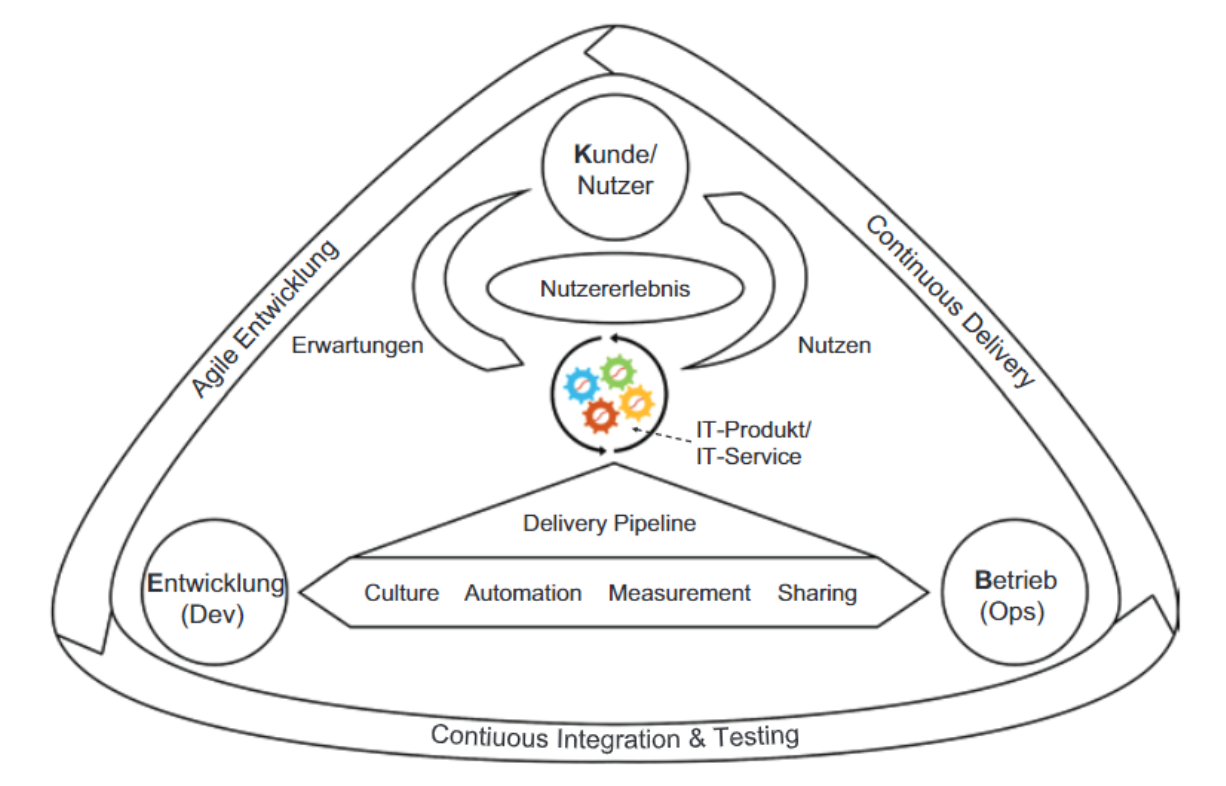
\includegraphics[width=1.0\textwidth]{gfx/devops_ueberblick.PNG}
 \caption{\citet{Alt2017}, S. 28, DevOps im Überblick\label{fig:devops}}
\end{figure}
\medskip
\\
Abb. \ref{fig:devops} stellt das DevOps Lebenszyklus mit ihren jeweiligen kontinuierlichen Verfahren dar, die das Produkt und die Beteiligten umfassen. Agile Entwicklung, \ac{CI} und \ac{CD} sind jeweils Verfahren, die vor DevOps existierten. Sie werden in diesem Zusammenhang jedoch als ein kontinuierliches Modell gesehen, die eine Schnittstelle zwischen den Beteiligten herstellt und das Produkt dadurch am Leben erhält und wachsen lässt. Das Wesentliche an diesem Modell ist ein Kontinuitätsprinzip \cite{Alt2017} der Prozesse auf allen Ebenen.

\paragraph{Infrastructure as Code}
\ac{IaC} ist die Abstraktion von IT-Infrastrukturen und -Ressourcen auf eine Ebene analog zu Quellcode. Diese Analogie impliziert schon eine Automatisierung in der Ausführung dieser Instruktionen. Die Bereitstellung von IT-Ressourcen kann aufgrund der steigenden Anforderungen an die IT-Architektur \cite{Brockhoff2006, Bussmann2006, Alt2017} nicht manuell erfolgen und muss automatisiert werden. Daher ist dieser Ansatz für die Umsetzung von DevOps erforderlich.

\paragraph{Infrastructure as a Service}
\ac{IaC} bietet eine Möglichkeit die IT-Architektur serviceorientiert aufzubauen. Daraus resultiert \ac{IaaS}, die sich darauf Konzentriert IT-Ressourcen dem Kunden nach Bedarf zur Verfügung zu stellen. Wenn der Bedarf sinkt, werden die Ressourcen an eine andere Stelle allokiert.

\paragraph{Cloud-Computing}

\paragraph{Software as a Service}

\paragraph{Platform as a Service}

\paragraph{Microservices}

\paragraph{Container-Virtualisierung}

\paragraph{Container-Orchestrierung}

\paragraph{ITIL}
Alt et al. beschreibt ITIL im Rahmen des Innovationsdrucks vom IT-Management:

Viele Organisationen haben ihre Leistungen nach dem ITIL-Service-Lebenszyklus strukturiert und den Ablauf an den ITIL-Prozessen ausgerichtet. ITIL bedingt die Kombination von Zweckmäßigkeit \enquote{Utility} und Einsatzfähigkeit \enquote{Warranty} für einen Wertbeitrag eines Services auf das Geschäft. Zweckmäßigkeit wird durch die Realisierung einer geforderten Funktion oder durch die Beseitigung einer Einschränkung erreicht. Als Qualitätsmerkmal gilt die Einsatzfähigkeit. Sie bezieht sich auf eine ausreichende Verfügbarkeit, Kapazität, Kontinuität und Sicherheit. Es ist Notwendig das bisherige Verständnis von IT-Services um das Kriterium \enquote{Innovationsbeitrag} zu ergänzen. Services müssen sich in einer Innovationskultur bezüglich ihres Beitrags zur Innovationsgenerierung messen lassen.

\cite{Alt2017}

\paragraph{Design Thinking}
Design Thinking ist ein Ansatz für einen Prozess für die Entwicklung von Produkten. Der Ablauf ihrer Schritte erfolgt iterativ. 

\paragraph{IT4IT}